\scanpage{357}
\uline{Th Eilenberg.Zilber-Cartier}\hfill EZ 1

$X_{**}$ un \deleted{groupe}\inserted{objet} abelien \unsure{bisimplicial|bisimplical} $(\qquad)$.
\deleted{\[
\unsure{N(\text{\unsure{bisimpl|bicompl}})\longrightarrow|N:\mathrm{Ab}(\text{bisimpl.})\longrightarrow A(}
\]}
\diagram{\begin{tikzcd}
N:A_{**}\arrow[r,"\text{eq de cat}","\sim"'] & A_{\bullet\bullet}\\
\widetilde{\phantom{X}}:A_{**}\arrow[r] & A_{\bullet\bullet}\\
\Delta:A_{**}\arrow[r] & A_*\\
\int:A_{\bullet\bullet}\arrow[r] & A_\bullet
\end{tikzcd}}
\margin{(complexe \unsure{associé|associe}}
\margin{\diagram{\begin{tikzcd}
N:A_*\arrow[r] & A_\bullet\\
\widehat{\phantom{X}}:A_*\arrow[r]&A_\bullet
\end{tikzcd}}
\diagram{\begin{tikzcd}
N\arrow[r,hook]&\widetilde{(\ )}\\
&D(\ )\arrow[u]
\end{tikzcd}}
\unsure{q ism|q isom}\quad degen \unsure{homot$^{\mathrm t}$|homot.} triv}

$\exists$ des \deleted{\unsure{quasi-iso|quasi iso} naturels}\inserted{morphismes} fonctoriels,
\diagram{\begin{tikzcd}
\int N\arrow[r,shift right,"\varphi"'] &N\Delta\arrow[l,shift right,"\psi"']
\end{tikzcd}}
\deleted{$\unsure{\psi|X}_{0,0}$}
qui coincident avec les fleches \unsure{evidentes|evidents} en degré 0.
\diagram{\begin{tikzcd}[row sep=small]
A_{**}\arrow[rr,"N"]\arrow[ddd,no head,"\Delta"]&&A_{\bullet\bullet}\arrow[ddd,"\int"]&\deleted{\longrightarrow}\\
&&{}\arrow[dl,bend right=25]&\\
&{}\arrow[ur,bend right=25]&&\\
A_*\arrow[rr,"N"]&&A_\bullet&
\end{tikzcd}}
\[
\varphi\psi\sim1_{\int N}\qquad\psi\varphi\sim1_{\unsure{N|\int}\Delta}
\]
\deleted{$\unsure{\varphi\psi\unsure{N|\int}(X_{**})}$}
\diagram{\begin{tikzcd}
\psi\varphi\int(\underbrace{NX_{**}})\arrow[r]&\int NX_{**}\\
\varphi\psi\underbrace{N\Delta}X_{**}\arrow[r]&N\Delta\unsure{X|\lambda}_{**}
\end{tikzcd}}
\[
1-\psi\varphi=dk+kd\qquad1-\varphi\psi=dh+hd
\]
\diagram{\begin{tikzcd}
k:\int NX_{**}\arrow[r,shift left,"+1"]\arrow[r,shift right,dashed]&\int N\unsure{X|\lambda}_{**}\\
&\colon\\
h:N\Delta X_{**}\arrow[r,"+1"]&N\Delta X_{**}
\end{tikzcd}}
\figure{\begin{tikzpicture}\draw (0,0)--(4,0);\end{tikzpicture}}
\diagram{\begin{tikzcd}
\int N\arrow[r,shift left,no head,"\psi"]\arrow[d,bend right=20]&N\Delta\arrow[l,shift left,"\varphi"]\arrow[d,bend right=20]\\
\int\widetilde{\phantom X}\arrow[r,shift left,"\widetilde\psi"]&\widetilde{\phantom X}\Delta\arrow[l,shift left,"\widetilde\varphi"]
\end{tikzcd}}
\deleted{$k-\unsure{k|h}'=$}
\diagram{\begin{tikzcd}
\int\widetilde{\phantom X}\arrow[r,shift right,"\widetilde\varphi"']&\widetilde{\phantom X}(\Delta)\arrow[l,shift right,"\widehat\psi"']
\end{tikzcd}}
Si $\varphi$ et $\psi$ sont choisis, Pour un autre choix de $k',h'$
\[
k'-k=d\ell+\ell d\qquad h'-h=dm+md
\]
etc\ldots\quad$\ell$ et $m$ fonct

$\exists$ des choix traditionnels: ``application d'Alexander Whitney''
\deleted{EZ 2}
``shuffles''

\uuline{\uline{cf MacLane}}\quad Homology
\diagram{\begin{tikzcd}
(\int\widetilde X_{**})_n=\displaystyle\bigoplus_{i+j=n}X_{(i)(j)}\arrow[r,"\text{shuffles}"]&\widetilde X_{(n,n)}\\
\underbrace{x_{ij}}\arrow[r]&\deleted{\unsure{\sum\delta s_\alpha s'_\beta|\sum\varepsilon s_\alpha s'_\beta(}}\quad x_{i+j,i+j}
\end{tikzcd}}
$(i,j)$-shuffle
\diagram{\begin{tikzcd}
(1\quad\ldots,\overset{\substack{n.\\\Vert}}{i+j})\arrow[d,no head]&{}\\
s(1)\quad\ldots\quad\underbrace{s(i)}\quad\underbrace{s(i+j)}&{}
\end{tikzcd}}
\[
x_{i1}\qquad x_{i+1,i+1}
\]
\[
\sum_{0\le\alpha\le i}\unsure{(-)|(\ )}s_\alpha s'_0s'_1\ldots
\overset{\deleted{\unsure{x_i|\wedge}}}{s_\alpha}\ldots s'_i\,x_{i1}
\]
\margin{signe$(\sigma)$}
\[
\sum_{\substack{\text{sur tout }\sigma\in\Sigma_n\\
\text{t.q }\sigma(\alpha)<\sigma(\beta)\\
\alpha<\beta\le i\ \text{ou}\ \deleted{\unsure{i+1\le|i+1<}}\ i<\alpha<\beta\le n.}}
\underbrace{s_{\sigma(i+1)}\ldots s_{\sigma(i+j)}}\,
\underbrace{s'_{\sigma(1)}\ldots s'_{\sigma(i)}}
\]
$\sigma\unsure{\mathbb Z|\Sigma}$
\figure{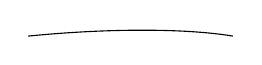
\begin{tikzpicture}\draw (0,0) .. controls (1,.1) and (2,.1) .. (2.6,0);\end{tikzpicture}}
\margin{Shuffles}
\figure{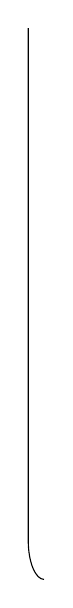
\begin{tikzpicture}
\draw (0,0)--(0,-6.5) .. controls (0,-6.8) and (.1,-7) .. (.2,-7);
\end{tikzpicture}}
\[
A\qquad\overline B(A)
\]
\diagram{\begin{tikzcd}[execute at end picture={\begin{scope}[x=.015cm,y=-.015cm]\node at (70,32) {$[n\deleted{\unsure{i|j}}]$};\node at (385,32) {$[i\deleted{\unsure{+j}}]$};\draw (60,93) .. controls (110,120) and (240,150) .. (335,219);\draw (50,128) .. controls (105,165) and (230,183) .. (290,227);\draw (50,158) .. controls (120,185) and (210,213) .. (259,219);\draw (43,186) .. controls (90,210) and (200,209) .. (229,225);\draw (54,203) .. controls (175,210) and (170,184) .. (339,199);\draw (65,245) .. controls (140,238) and (230,247) .. (343,243);\draw (50,288) .. controls (130,284) and (235,282) .. (340,275);\draw (33,331) .. controls (160,306) and (250,307) .. (333,315);\draw (65,363) .. controls (190,344) and (290,367) .. (395,361);\node at (340,196) {$\unsure{2|\bullet}$};\node at (342,253) {$\unsure{?|1}$};\node at (342,293) {$\unsure{i|\vdots}$};\node at (340,330) {$0$};\draw (49,147)--(47,151);\draw (50,155)--(48,160);\draw (49,201)--(50,211);\fill (49,225) circle[radius=1.3];\draw (46,269)--(48,254)--(51,257);\draw (46,315)--(44,309);\draw (47,322)--(45,326);\fill (36,342) circle[radius=.8];\end{scope}}]\phantom A\end{tikzcd}}

\uuline{Alexander-Whitney}
\diagram{\begin{tikzcd}
\widehat X_{n,n}\arrow[r]&\bigoplus X_{ij}\\
x_{n,n}\arrow[r]&\displaystyle\sum_{i=0}^n(-1)^i d_0^{n-i}\widehat d^{\prime i}X_{n,n}
\end{tikzcd}}
\diagram{\begin{tikzcd}[column sep=small]
\underset{f}{\underbrace{C^i(X,A)}}\otimes\underset{g}{\underbrace{C^j(X,B)}}\arrow[r,phantom,"{\unsure{\Rightarrow|\rightarrow}}" description]&\underbrace{C^{i+j}(X\times X,A\otimes B)}\arrow[r,bend right=15]&C^{i+j}(X,A\otimes B\\
ZX\otimes ZX&\underbrace{Z(X\times X)}\arrow[l,phantom,"{\unsure{\Leftarrow|\leftarrow}}" description]&{}
\end{tikzcd}}
$\widehat d$ signifie le dernier op face

$d'$ seconde op simpl.
\[
\widehat d^{\prime i}=\underbrace{d^{\prime n}d^{\prime n-1}\ldots d^{\prime n-i+1}}
\]
\[
\mathrm{E\!-\!Z\!-\!C}\mathrel{\vert\!\Rightarrow}\mathrm{E\!-\!Z}
\]
Cup-produit
\[
\left\{\begin{aligned}
h(x_1\ldots,x_{\unsure{n+1|n,1}})\\
{}=\sum\unsure{(-i)|(-1)}f(x_1\ldots,x_i)g(x_{i+1},\ldots x_n)
\end{aligned}\right.
\]
\margin{\figure{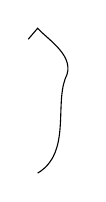
\begin{tikzpicture}
\draw (0,0) .. controls (.42,.25) and (.22,.85) .. (.35,1.2) .. controls (.5,1.48) and (.12,1.7) .. (0,1.84)--(-.12,1.7);
\end{tikzpicture}}}
\uline{Associatif}\quad(non-commutatif mais comm à homotopie près)
\[
\Rightarrow H^*(X,R)\quad\text{est anticom.}
\]
\mspage{358}
